\chapter{Nonlinear differential script}
\label{NLDS}
The nonlinear differential script contains all the information about the system and how it is constructed. The model needs 8 different inputs(u): 
the opening degree of the 4 PMA valves and the differential pressure across the main and PMA pumps. This inputs are obtained from the lab and are 
inserted directly into the model. Furthermore, it has been decided to include the dynamics of the system so the model remains as a nonlinear differential system. 

First, the states of the system are set. Previously in the report, the states have been defined as the chord flows and denoted as $z = [z_1 z_2 z_3 z_4 z_5 z_6 
z_7]$. The value of the states will be dependent on time, which will be specified by the data obtained from the Water Wall Setup in the lab. In this way, using
the relation stated in \eqref{ChordRelation} the flow through the edges is obtained.

The pressure across the edges has been defined in \eqref{ComponentFunction}, and in the same way has been done in Matlab. 

\begin{itemize}
  \item $\lambda$ and $\zeta$ denote the pressure in the pipes due to the friction and the elevation respectively.
  \item $\nu$ represents the pressure across the valves.
  \item $\alpha$ represent the pressure across the pumps, which is obtained from the inputs to the model.
\end{itemize}

In the system in total there are 15 pipes, the pressure across them is obtained as: 

\begin{equation}
\lambda = (C_p * abs(q)*q /(10^5*3600^2)) + ((Z)*g*1000/10^5)
\end{equation}

Where, $C_p$ denotes the friction coefficient to be estimated by the NonLinear Grey Box and $Z$ is the height of the pipes. An initial guess is done for the value of $C_p$ to minimize the error 
as possible. Moreover, the unit conversion from Bar to Pas and seconds to hours is introduced.

\begin{equation}
  Cp= f*((8*L*rho)/(pi^2*D^5))+k_f*((8*rho)/(pi^2*D^4))
\end{equation}

The $f$ and $k_f$ values are obtained as described in \eqref{turbulent} and \eqref{kfriction} with the range of values considered in \secref{FormResistance}.

In case of the valves the pressure across them is obtained as following

\begin{equation}
  mu = (1/C_v^2)* abs(q)*q /3600^2;
\end{equation}

The value of $C_v$ is obtained from the input data. When the valve is closed $\mu$ is set to 0. 

For the pumps, the pressure across them is obtained from the lab and is set as $\alpha$. 

As pointed out earlier, the inertia of the pipes is taken into account in the model and is calculated as

\begin{equation}
  J = diag((4*L*rho)/(D^2*pi*10^5*3600));
\end{equation}

Where, $L$ and $D$ are the pipes length and diameters respectively. The unit conversion is also added. 

A new matrix variable is defined containing the pressure across the edges.

\begin{equation}
  F = \lambda + \mu - \alpha
\end{equation}

The derivative of the chords can be obtained isolating $\dot{z}$ in \eqref{isolateZ}

\begin{equation}
  \dot{z}  =  - (B_1 J {B_1}^T)^{-1}B_1 F
  \label{chordder}
\end{equation}

Where, $B_1$ is the cycle matrix defined in \appref{CycleAppendix}. 

Known the derivative of the chords, the derivative of the flow through the edges is obtained

\begin{equation}
  \dot{q}  = (B_1)^T * \dot{z}
  \label{flowder}
\end{equation}

\eqref{ChordsModel} is now applied substituting $\dot{q}$ with the relations set in \eqref{flowder} and \eqref{chordder}, resulting in

\begin{equation}
  \Delta P = [(J*(B_1)^T * (B_1 J {B_1}^T)^{-1}B_1 (-\mu - \lambda + \alpha)]+\mu+\lambda-\alpha
  \label{DeltaP}
\end{equation}

Now the pressure across the edges are calculated, nevertheless, from the data of the lab the relative pressure at the nodes are obtained. This implies to 
have to calculate the pressure in the nodes so the comparison is done correctly. 

The pressure at each node can be found by applying 

\begin{equation}
  \Delta P = (H_1)^T p
\end{equation}

$\Delta P$ is known from \eqref{DeltaP}, the vector of pressure in the nodes is split up as $p = [p_o \quad p_r]$ where $p_o$ is the atmospheric pressure at 
node 1 and $p_r$ the pressure in the remaining nodes. Splitting $H_1$ matrix also

\begin{equation}
  \Delta P = [{H_o}^{T} \quad {H_r}^{T}] 
  \begin{bmatrix}
    p_o \\
    p_r
  \end{bmatrix}
\end{equation}

Isolating $p_r$ from the equation the pressure at each node is obtained

\begin{equation}
  p_r = H_r^{\dagger} (\Delta p - (H_o)^{T} p_o)
\end{equation}

$H_r^{\dagger}$ being the pseude-inverse of matrix ${H_r}^{T}$.

The outputs are set as node 2, node 4, node 5, node 7, node 10, node 11, node 15 and node 16 (see \appref{systemdiagram} for the notation). Which will be the ones that Matlab will try to fit 
to the data obtained from the setup. 


%DO a NICE PLOT OF THIS!
%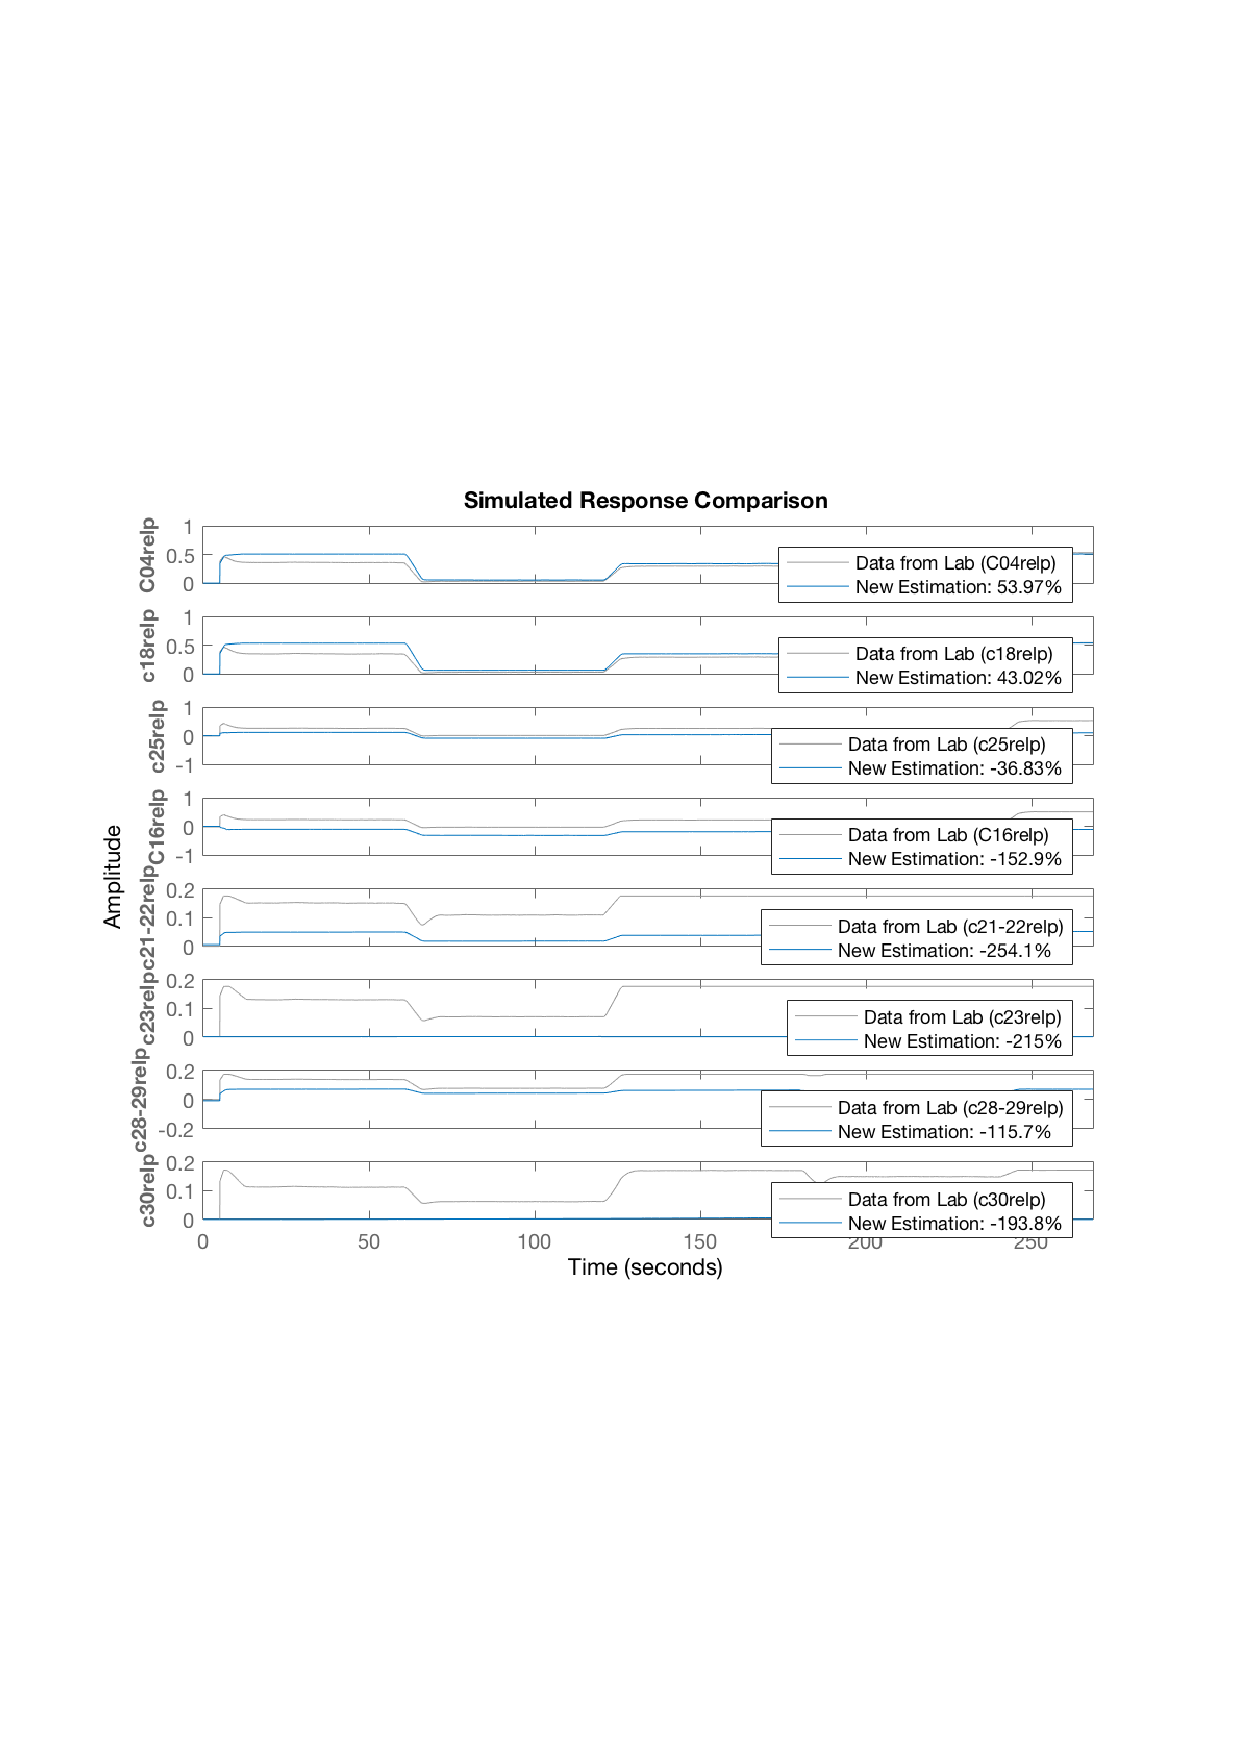
\includepdf[pages=-]{report/pictures/ComparePlot.pdf} 